\documentclass{ikpKoeln}
\usepackage{graphicx}
\usepackage{physics}
\usepackage{xcolor}
\usepackage{amsmath, bm}
\usepackage{tabularx}
\usepackage{array, arydshln}
\usepackage{tikz}
% \usepackage{enumitem}
\usetikzlibrary{math}

\scTitle{NeuLAND calibration revisit: Millepede algorithm and error analysis of map2cal calibration}
\scAuthor{*}{Yanzhao}{Wang}{1}
\scAffiliation{1}{University of Cologne, Institute for Nuclear Physics, Germany}

\scTitleShort{NeuLAND Meeting 05.04.2024}

\date{\scriptsize NeuLAND weekly meeting \\ 05.04.2024}

\graphicspath{{../figures/}}

\addbibresource{reference.bib}

\newcommand{\espeed}{C^i_e}
\newcommand{\espeedi}{C^i_{e0}}
\newcommand{\tspeed}{C^i_t}
\newcommand{\tsync}{t^i_{\text{sync}}}
\newcommand{\toff}{t^i_{\text{offset}}}

\begin{document}

\begin{frame}{Overview}
	\begin{itemize}
		\Large
		\setlength\itemsep{2em}
		\item Statistical error analysis of TDC calibration
		\item Millepede algorithm principle
		\item Millepede algorithm application to NeuLAND
		\item Preliminary results
	\end{itemize}
\end{frame}

\begin{frame}[t]{NeuLAND TDC calibration}
	\vspace*{-0.5em}
	\begin{columns}[t]
		\begin{column}{0.45\textwidth}
			\vspace*{-2em}
			\begin{block}{TDC calibration relation:}
				\small
				$f(x)$: Channel number $\Longrightarrow$ Time value (ns)
			\end{block}
			\begin{figure}
				\includegraphics[width = \textwidth]{ neulandMeeting/mapcal_plane_distri.png}
				\vspace*{1em}
				\includegraphics[width = \textwidth]{ neulandMeeting/mapcal_bar_dsistri.png}
			\end{figure}
		\end{column}
		\begin{column}{0.45\textwidth}
			\textit{\small Two time components:}
			\begin{itemize}
				\scriptsize
				\item coarse time ($\pm$ 5 ns)
				\item fine time ($\pm$ 10 ps)
			\end{itemize}
			\textit{\small Fine time Calibration procedures:}
			\begin{enumerate}
				\scriptsize
				\item Collection of of all TDC values
				\item Calculation of cumulative distribution of TDC values
				\item Scaling of CFD to $0\sim5$ ns
			\end{enumerate}
			\vspace*{-1em}
			\flushleft \scriptsize{CDF:}
			\begin{figure}
				\vspace*{-1em}
				\includegraphics[width = \textwidth]{ neulandMeeting/mapcal_cumulative.png}
			\end{figure}
		\end{column}
	\end{columns}
\end{frame}

\begin{frame}[t]{Statistical error analysis of TDC calibration}
	\flushleft \textbf{Convolution of two distributions:}
	\begin{itemize}
		\item Uniform distribution: fine time $\sim \mathcal{U}(f(n), f(n + 1))$
		\item Multinomial distribution: $f(n), f(n+1) \sim \mathcal{M}_k(3,p_a, p_b), \ p_a = \text{CDF}(n), p_b = \text{PDF}(n)$
	\end{itemize}

	\pause
	\flushleft \textbf{Mathematical derivation:}
	\flushleft {\small Mean:}
	\scriptsize{
		$$ E(X) = \sum_{n_a, n_b} \mathcal{M}(n_a,n_b;3,p_a, p_b) \cdot \int_{n_a}^{n_b} xf(x) \,dx = \bar{n_a} + \bar{n_b} / 2 $$
	}
	\flushleft {\small Variance:}
	{
		\scriptsize
		\begin{align*}
			Var(X) & = E(X^2) - E^2(X)                                                                                                                                                      \\
			E(X^2) & = \sum_{n_a, n_b} \mathcal{M}(n_a,n_b;3,p_a, p_b) \cdot \int_{n_a}^{n_b} x^2f(x) \,dx = \sum_{n_a, n_b} \mathcal{M}(n_a,n_b;3,p_a, p_b)(n_a^2n_b + n_an_b^2 + n_b^2/3) \\
			       & = Var(N_a) + E^2(N_a) + Cov(N_a, N_b) + E(N_a)E(N_b) + \left(Var(N_a) + E^2(N_b)\right)/3                                                                              \\
			Var(X) & = N^2 p_b^2 / 12 + N \left( -(p_a - \frac{1-p_b}{2})^2 + 1/4 - p_b / 6 - p_b^2 /12 \right)
		\end{align*}
	}%

\end{frame}

\begin{frame}[t]{Validation of the error analysis}
	\begin{columns}[t]
		\begin{column}{0.5\textwidth}
			\begin{alertblock}{\small Exact solution (no approximation):}
				\centering
				\small$\delta = \sqrt{\frac{N^2p_b^2}{12} + N \left( -(p_a - \frac{1-p_b}{2})^2 + \frac{1}{4} - \frac{p_b}{6} - \frac{p_b^2}{12} \right)}$
			\end{alertblock}
			\begin{exampleblock}{\small Approximate solution:}
				\centering
				\small$\delta = \frac{Np_b}{\sqrt{12}} + \frac{\sqrt{3}}{p_b}(-(p_a - \frac{1}{2})^2 + \frac{1}{4})$ \,\,\, ($p_b \neq 0$)
			\end{exampleblock}
			\begin{block}{\small Base solution:}
				\centering
				\small$\delta = \frac{Np_b}{\sqrt{12}}$
			\end{block}
		\end{column}
		\begin{column}{0.45\textwidth}
			\vspace*{-1.5em}

			\flushleft \textit{Comparison to Monte-Carlo data:}
			\begin{figure}
				\includegraphics[width = \textwidth]{ neulandMeeting/mapcal_error_validation.png}
			\end{figure}
			\vspace*{-2em}
			{
				\small
				\begin{flalign*}
					p_b & : 0.01    & \\
					N   & : 100'000 & \\
				\end{flalign*}
			}
		\end{column}
	\end{columns}
\end{frame}

\begin{frame}[t]{NeuLAND time and position calibration}
	\vspace*{-2em}
	\begin{columns}[t]
		\begin{column}{0.45\textwidth}
			\begin{block}{\small Time relation:}
				\centering
				$ t = \frac{t_r + t_l}{2} - \frac{L}{2 \cdot \alert{C_e}} + \alert{t_\text{sync}}$
			\end{block}

			\begin{block}{\small Position relation:}
				\centering
				$ x = \frac{\alert{C_e}}{2}\left( t_r - t_l  + \alert{t_\text{offset}} \right)$
			\end{block}
			\flushleft\textbf{Calibration parameters:}
			\begin{itemize}
				\item \alert{$C_e$}  : effective speed of light
				\item \alert{$t_\text{sync}$} : time synchronization among scintillators
				\item \alert{$t_\text{offset}$} : time offset between adjacent PMTs
			\end{itemize}

		\end{column}
		\pause
		\begin{column}{0.45\textwidth}
			\flushleft\textbf{Calibration using muon tracks:}
			\begin{block}{\small Time and position relation for muon tracks:}
				\centering
				\vspace*{-1.5em}
				\begin{align}
					\small
					x_\mu & = \textcolor{blue}{a^i_x} \cdot z_\mu  + \textcolor{blue}{b^i_x} \\
					y_\mu & = \textcolor{blue}{a^i_y} \cdot z_\mu  + \textcolor{blue}{b^i_y} \\
					t_\mu & = \textcolor{blue}{a^i_t} \cdot z_\mu  + \textcolor{blue}{b^i_t}
				\end{align}
			\end{block}
			\flushleft\textit{\small Calibration parameters for the $j$th muon track in $i$th bar:}
			$$\alert{C^i_e}, \alert{t^i_\text{sync}}, \alert{t^i_\text{offset}},\textcolor{blue}{a^j_x}, \textcolor{blue}{a^j_y}, \textcolor{blue}{a^j_t}, \textcolor{blue}{b^j_x}, \textcolor{blue}{b^j_y}, \textcolor{blue}{b^j_t} $$
			\flushleft\textit{\small Total number of calibration parameters for $n$ muon tracks:} $ 3900 + 6n$
		\end{column}
	\end{columns}
\end{frame}

\begin{frame}[t]{Principle of Millepede algorithm}
	\vspace*{-2em}
	\begin{columns}[t]
		\begin{column}{0.45 \textwidth}
			\onslide<1->
			\begin{center}
				\textbf{Linear regression}
			\end{center}
		\end{column}
		\begin{column}{0.45 \textwidth}
			\onslide<2>
			\begin{center}
				\textbf{Newton's method}
			\end{center}
		\end{column}
	\end{columns}
	\begin{columns}[t]
		\begin{column}{0.45 \textwidth}
			\onslide<1->
			\begin{block}{\small Residual minimization}
				\vspace{-1em}
				$$\large{\partial} \sum^n_{j = 1}\sum^{b(j)}_{i = 1} \frac{(\mathcal{Z}^j_i(g_1, ..., g_m, p^j_1, ..., p^j_l))^2}{ 2 (\sigma^j_i)^2} = 0$$
			\end{block}
			{\scriptsize
			\begin{flalign*}
				\mathcal{Z}^j_i & : \text{Residual values (linear) for $j$th track and $i$th bar}  & \\
				g_{1\ldots m}   & : \text{$m$ \textit{global parameters}}                          & \\
				p^j_{1\ldots l} & : \text{$l$ \textit{local parameters} for the $j$th $\mu$ track} & \\
				n               & : \text{the total number of $\mu$ tracks}                        & \\
				b(j)            & : \text{the total number of bars for the $j$th $\mu$ track}      &
			\end{flalign*}

			\vspace*{-1em}
			}
		\end{column}
		\begin{column}{0.45 \textwidth}
			\onslide<2>
			\begin{itemize}
				\setlength{\itemindent}{-1em}
				\item \textit{\small Single variable:}
				      \begin{columns}
					      \begin{column}{0.6\textwidth}
						      \begin{figure}
							      \includegraphics[width = \textwidth]{neulandMeeting/Newton_iteration.png}
						      \end{figure}
					      \end{column}
					      \begin{column}{0.4\textwidth}
						      \begin{align*}
							      \delta x & = x_{n+1} - x_n     \\
							               & = -f(x_n) / f'(x_n)
						      \end{align*}
					      \end{column}
				      \end{columns}
				\item \textit{\small Multivariable:}
				      \vspace*{-1em}
				      $$\nabla f(\vec{x}_n) \cdot \delta \vec{x} = -f(\vec{x}_n)$$
			\end{itemize}

			\flushleft {\vspace*{-0.5em} \textbf{Residual minimization:}}
			\vspace*{-1em}
			\begin{align*}
				\nabla \vec{f}(\vec{x}_n) & = \nabla(\nabla \mathcal{F}(g_1, ..., g_m, p^j_1, ..., p^j_l)) \\
				                          & = \textsc{H}\mathcal{F}(g_1, ..., g_m, p^j_1, ..., p^j_l))
			\end{align*}

			% \flushleft \textit{\small Single variable:}
			% \vspace*{-1em}
			% \begin{columns}
			% 	\begin{column}{0.6\textwidth}
			% 		\begin{figure}
			% 			\includegraphics[width = \textwidth]{neulandMeeting/Newton_iteration.png}
			% 		\end{figure}
			% 	\end{column}
			% 	\begin{column}{0.4\textwidth}
			% 		\begin{align*}
			% 			\delta x & = x_{n+1} - x_n     \\
			% 			         & = -f(x_n) / f'(x_n)
			% 		\end{align*}
			% 	\end{column}
			% \end{columns}
			% \flushleft \textit{\small Multivariable:}
			% \vspace*{-1em}
			% $$\nabla f(\vec{x}_n) \cdot \delta \vec{x} = -f(\vec{x}_n)$$
			% \flushleft {\vspace*{-0.5em} \textbf{Residual minimization:}}
			% \vspace*{-1em}
			% \begin{align*}
			% 	\nabla \vec{f}(\vec{x}_n) & = \nabla(\nabla \mathcal{F}(g_1, ..., g_m, p^j_1, ..., p^j_l)) \\
			% 	                          & = \textsc{H}\mathcal{F}(g_1, ..., g_m, p^j_1, ..., p^j_l))
			% \end{align*}
		\end{column}
	\end{columns}
\end{frame}

\begin{frame}[t]{Principle of Millepede algorithm}
	\vspace*{-0.9em}
	\begin{columns}[t]
		\begin{column}{0.5 \textwidth}
			\begin{block}{\small Hessian operation (second derivative matrix)}
				\centering
				$\left[\textsc{H} \mathcal{F}(x_1, x_2, \cdots, x_n)\right]_{ij} = \frac{\partial^2\mathcal{F}}{\partial x_i \partial x_j} \sim \sum\frac{\partial \mathcal{Z}}{\partial x_i}\frac{\partial \mathcal{Z}}{\partial x_j}$
			\end{block}
			\textbf{\small Using Newton's method:}
			\begin{center}
				$\left[\textsc{H} \mathcal{F}(\boldsymbol{x})\right]\Delta\boldsymbol{x} = - \nabla \mathcal{F}(\boldsymbol{x})$
			\end{center}
			% \vspace*{-1em}
			\hspace{3pt}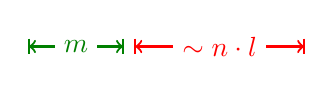
\begin{tikzpicture}[thick]
				\tikzset{good one/.style={color=black!50!green}}
				\draw[good one] (-0.3, 0.1) -- (-0.3, -0.1);
				\draw[<->,good one] (-0.3, 0) -- node[fill=white]{$m$}(0.9, 0);
				\draw[good one] (0.9, 0.1) -- (0.9, -0.1);

				\draw[red] (1.05, 0.1) -- (1.05, -0.1);
				\draw[<->,red] (1.05, 0) -- node[fill=white]{$\sim n \cdot l$}(3.2, 0);
				\draw[red] (3.2, 0.1) -- (3.2, -0.1);
			\end{tikzpicture}
			\vspace*{-0.9em}
			\setlength\extrarowheight{6pt}
			\scriptsize{
				$$ \left[  \begin{array}{c||c:c:c}
							\sum_j \mathcal{C}_j & \ldots & \mathcal{G}_j & ...    \\[6pt] \hline\hline
							\vdots               & \ddots & 0             & 0      \\[4pt] \hdashline
							\mathcal{G}^T_j      & 0      & \Gamma_j      & 0      \\[6pt] \hdashline
							\vdots               & 0      & 0             & \ddots \\
						\end{array}  \right] \cdot
					\left[ \begin{array}{c}
							\alert{\Delta \mathbf{g}} \\[6pt] \hline\hline
							\vdots                    \\[4pt] \hdashline
							\Delta \mathbf{p}^j       \\[6pt] \hdashline
							\vdots                    \\
						\end{array} \right] =
					-\left[ \begin{array}{c}
							\sum_j\partial_\mathbf{g} \mathcal{F}_j \\[6pt] \hline\hline
							\vdots                                  \\[4pt] \hdashline
							\partial_{\mathbf{p}^j} \mathcal{F}     \\[6pt] \hdashline
							\vdots                                  \\
						\end{array} \right]
				$$
			}
		\end{column}
		\pause
		\begin{column}{0.4 \textwidth}
			\textbf{\textit{Schur complement method:}}
			$$\tilde{\mathcal{C}} \cdot \Delta \mathbf{g} = \mathcal{D}$$
			\vspace*{-1.5em}

			where
			\vspace*{-1.5em}

			\begin{align*}
				\tilde{\mathcal{C}} & = \sum_j \mathcal{C}_j + \sum_j \left(-\mathcal{G}_j \Gamma^{-1}_j \mathcal{G}^T_j \right)                       \\
				\mathcal{D}         & = \sum_j\partial_\mathbf{g} \mathcal{F}_j - \sum_j\mathcal{G}_j \Gamma^{-1}_j\partial_{\mathbf{p}^j} \mathcal{F}
			\end{align*}
			\vspace*{-1.5em}

			\begin{exampleblock} {Advantages}
				\small
				\begin{itemize}
					\item Simultaneous fitting of all parameters
					\item Computation complexity independent of local parameter size
					\item No muon track reconstruction
				\end{itemize}
			\end{exampleblock}
		\end{column}
	\end{columns}
\end{frame}

\begin{frame}{Millepede algorithm for NeuLAND}
	\vspace*{-2em}
	\begin{columns}[t]
		\begin{column}{0.45 \textwidth}
			\onslide<1->
			\begin{center}
				\textbf{Residual equations for NeuLAND}
			\end{center}
		\end{column}
		\begin{column}{0.45 \textwidth}
			\onslide<2>
			\begin{center}
				\textbf{Linearization}
			\end{center}
		\end{column}
	\end{columns}
	\begin{columns}[t]
		\begin{column}{0.5 \textwidth}
			\onslide<1->
			\setcounter{equation}{0}
			{\small
				\begin{block}{For horizontal bars}
					\centering
					\vspace*{-1em}
					\begin{align}
						0              & = b_x + \espeed \toff/ 2 + \espeed \Delta t/2 + a_x z_i \\
						t_\text{sum}/2 & =b_t + \frac{L}{2 \espeed}  + \tsync + a_t z_i          \\
						y_i            & = b_y + a_y z_i
					\end{align}
				\end{block}
				\begin{block}{For vertical bars}
					\centering
					\vspace*{-1em}
					\begin{align}
						0              & = b_y + \espeed \toff/ 2 + \espeed \Delta t /2 + a_y z_i \\
						t_\text{sum}/2 & =b_t + \frac{L}{2 \espeed}  + \tsync + a_t z_i           \\
						y_i            & = b_x + a_x z_i
					\end{align}
				\end{block}
			}
		\end{column}
		\begin{column}{0.45 \textwidth}
			\onslide<2>
			\begin{itemize}
				\item {\scriptsize Parameter redefinition $\tspeed \equiv \espeed \toff$ in Eq. (1, 4):}
				      \vspace*{-0.5em}
				      \begin{align*}
					      0 & = b_x + \espeed \toff/ 2 + \espeed t_\text{diff}/2 + a_x z_i \\
					        & = b_x + \tspeed/ 2 + \espeed t_\text{diff}/2 + a_x z_i
				      \end{align*}
				\item {\scriptsize Taylor expansion of $\espeed$ near $\espeedi$ in Eq. (2, 5):}
				      \vspace*{-0.5em}
				      \begin{align*}
					       & t_\text{sum}/2  =b_t + \frac{L}{2 \espeed}  + \tsync + a_t z_i                                     \\
					       & \sim b_t + L \left( \frac{1}{\espeedi} - \frac{\espeed}{2(\espeedi)^2} \right)  + \tsync + a_t z_i
				      \end{align*}
			\end{itemize}
		\end{column}
	\end{columns}
\end{frame}

\begin{frame}{First order derivatives of residual equations}
	\setlength\arraycolsep{1pt}
	\renewcommand{\arraystretch}{1.}
	\flushleft \textbf{\textit{Derivatives of all parameters for $i$th bar:}}
	$$
		\begin{array}{c||c|c|c|c|c|c||c|c|c|c|c|c|c|c}
			\text{Eq.} & a_x & a_y & a_t & b_x & b_y & b_t & \tsync\text{\tiny(H)} & \tsync\text{\tiny(V)} & \tspeed \text{\tiny(H)} & \tspeed \text{\tiny(V)} & \espeed \text{\tiny(H)}   & \espeed  \text{\tiny(V)}  & \text{meas}                                 & \text{err}                             \\ \hline
			\text{(1)} & z_i & 0   & 0   & 1   & 0   & 0   & 0                     & 0                     & \frac{1}{2}             & 0                       & \frac{t_\text{diff}}{2}   & 0                         & 0                                           & \frac{\espeedi}{2}\delta t_\text{diff} \\
			\text{(4)} & 0   & z_i & 0   & 0   & 1   & 0   & 0                     & 0                     & 0                       & \frac{1}{2}             & 0                         & \frac{t_\text{diff}}{2}   & 0                                           & \frac{\espeedi}{2}\delta t_\text{diff} \\
			\text{(2)} & 0   & 0   & z_i & 0   & 0   & 1   & 1                     & 0                     & 0                       & 0                       & -\frac{L}{2 (\espeedi)^2} & 0                         & \frac{t_{\text{sum}}}{2}-\frac{L}{\espeedi} & \frac{1}{2}\delta t_{\text{sum}}       \\
			\text{(5)} & 0   & 0   & z_i & 0   & 0   & 1   & 0                     & 1                     & 0                       & 0                       & 0                         & -\frac{L}{2 (\espeedi)^2} & \frac{t_{\text{sum}}}{2}-\frac{L}{\espeedi} & \frac{1}{2}\delta t_{\text{sum}}       \\
			\text{(3)} & 0   & z_i & 0   & 0   & 1   & 0   & 0                     & 0                     & 0                       & 0                       & 0                         & 0                         & y_i                                         & w_{\text{\tiny bar}}                   \\
			\text{(6)} & z_i & 0   & 0   & 1   & 0   & 0   & 0                     & 0                     & 0                       & 0                       & 0                         & 0                         & x_i                                         & w_{\text{\tiny bar}}                   \\
		\end{array}
	$$

	{\small
			Variable names:
			\vspace*{-2em}

			\begin{columns}[t]
				\begin{column}{0.4\textwidth}
					\begin{flalign*}
						t_{\text{sum}}         & : \text{Summation of the adjacent PMT times}   & \\
						t_{\text{diff}}        & :  \text{Difference of the adjacent PMT times} & \\
						\delta t_{\text{sum}}  & : \text{Error value of $t_{\text{sum}}$}       & \\
						\delta t_{\text{diff}} & :  \text{Error value of $t_{\text{diff}}$}     & \\
					\end{flalign*}
				\end{column}
				\begin{column}{0.4\textwidth}
					\begin{flalign*}
						w_{\text{\tiny bar}} & : \text{Width of the $i$th bar}                    & \\
						x_i, y_i, z_i        & :  \text{$x$, $y$, $z$ positions of the $i$th bar} & \\
					\end{flalign*}
				\end{column}

			\end{columns}
		}
\end{frame}

\begin{frame}{Integration with \textsc{R3BRoot}}
	\begin{figure}
		\includegraphics[width = \textwidth]{neulandMeeting/millepede_integration.png}
	\end{figure}
\end{frame}

\begin{frame}{Preliminary results from Millepede algorithm}
	\begin{figure}
		\centering
		Comparison of the PMT time offset parameter
		\includegraphics[width = 0.7\textwidth]{neulandMeeting/t_diff.png}
	\end{figure}
\end{frame}
\begin{frame}{Preliminary results from Millepede algorithm}
	\begin{figure}
		\centering
		Comparison of the scintillator time synchronization
		\includegraphics[width = 0.7\textwidth]{neulandMeeting/tsync.png}
	\end{figure}
\end{frame}
\begin{frame}{Preliminary results from Millepede algorithm}
	\begin{figure}
		\centering
		Comparison of the scintillator effective of c
		\includegraphics[width = 0.7\textwidth]{neulandMeeting/effective_c.png}
	\end{figure}
\end{frame}
\end{document}
